\section{Supplementaries} \label{GLOBALsec:supplementaries}

table with bands by n, e, 

\subsection{Scaling}

% Expanded states
\begin{figure}[t]
    \centering
    \subfloat[$e=1\%, \spot=1$]{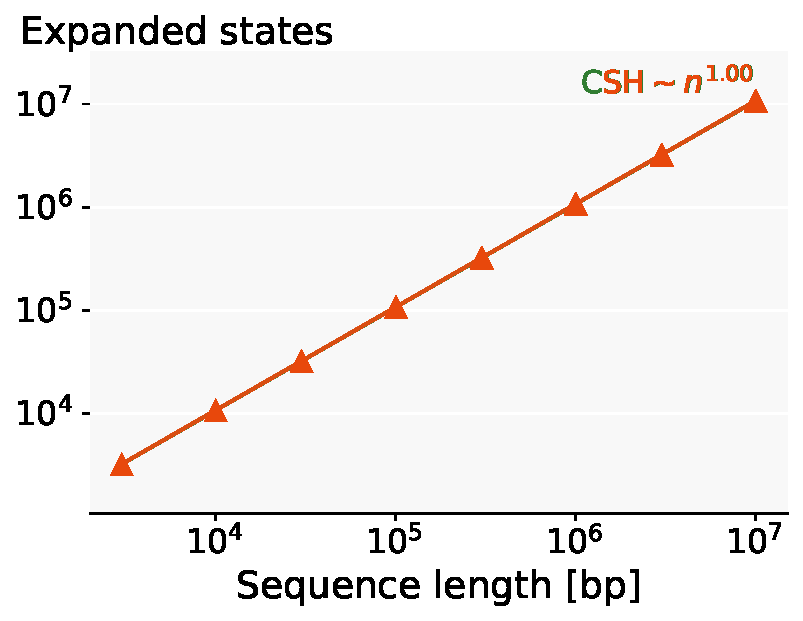
\includegraphics[width=0.5\linewidth]{imgs/scaling/expanded_e0.01.pdf}}
    \subfloat[$e=5\%, \spot=1$]{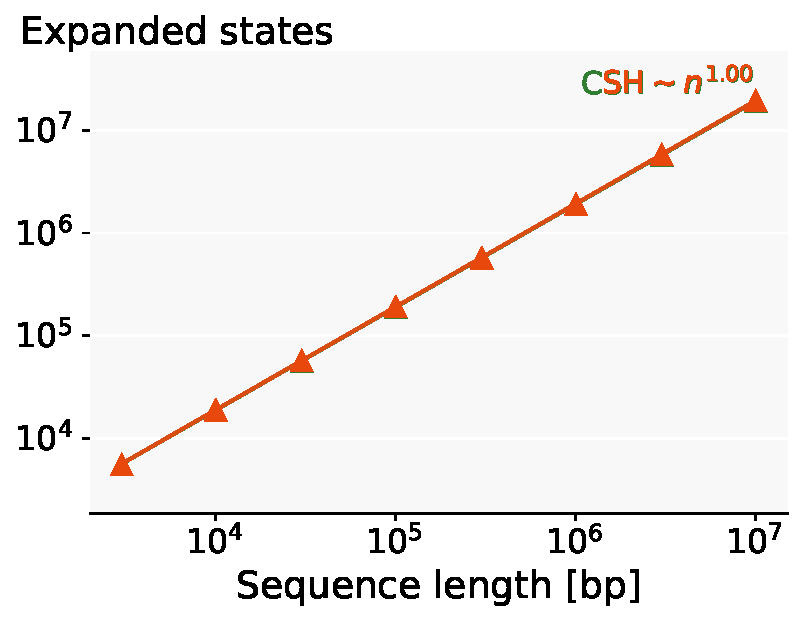
\includegraphics[width=0.5\linewidth]{imgs/scaling/expanded_e0.05.pdf}}\\
    \subfloat[$e=10\%, \spot=2$]{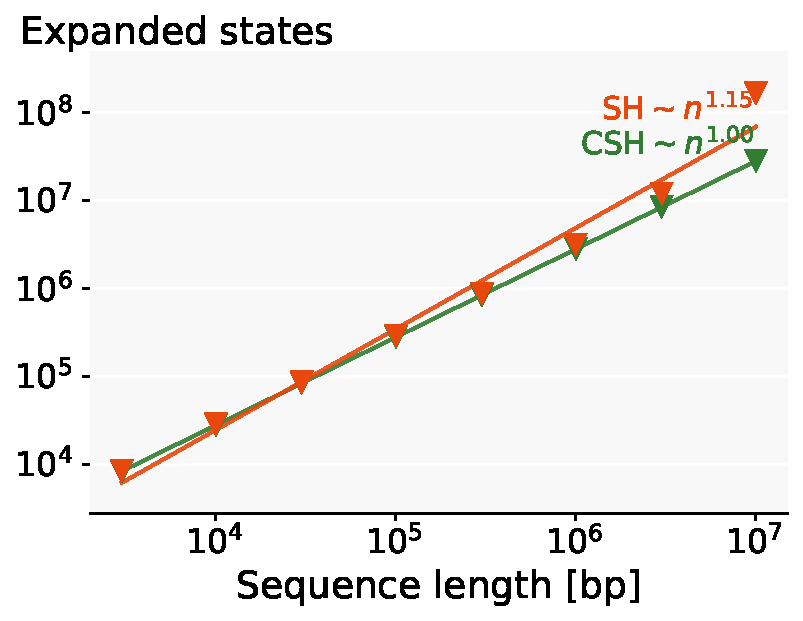
\includegraphics[width=0.5\linewidth]{imgs/scaling/expanded_e0.1.pdf}}
    \subfloat[$e=15\%, \spot=2$]{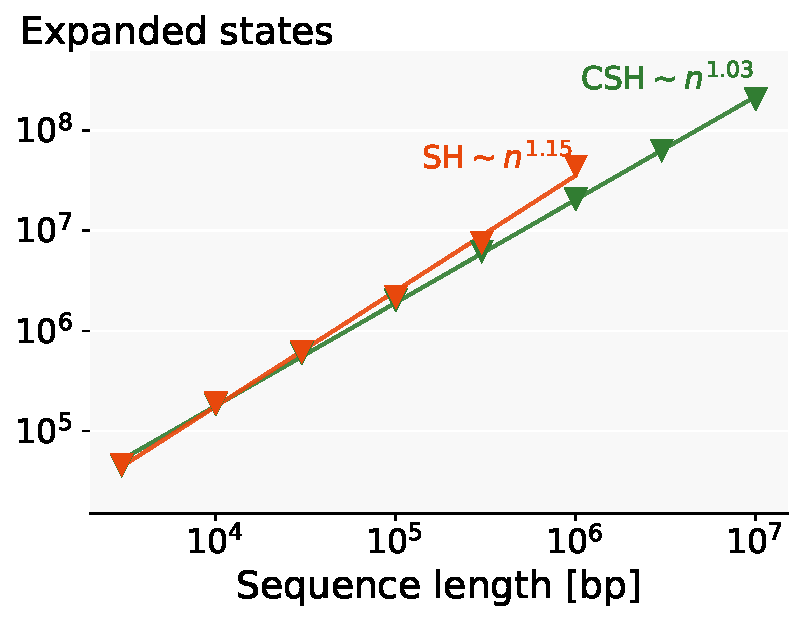
\includegraphics[width=0.5\linewidth]{imgs/scaling/expanded_e0.15.pdf}}
    \caption{Expanded states scaling. Polynomial fit. Note that $e$ is the
      generated errors, which is higher than the resulting difference.
      Note that for $e=20\%$ all \A solutions are quadratic too.}
    \label{GLOBALfig:expanded_length_scaling}
\end{figure}

% Memory
\begin{figure}[t]
    \centering
    \subfloat[$e=1\%, \spot=1$]{\includegraphics[width=0.5\linewidth]{imgs/scaling/memory_e0.01.pdf}}
    \subfloat[$e=5\%, \spot=1$]{\includegraphics[width=0.5\linewidth]{imgs/scaling/memory_e0.05.pdf}}\\
    \subfloat[$e=10\%, \spot=2$]{\includegraphics[width=0.5\linewidth]{imgs/scaling/memory_e0.1.pdf}}
    \subfloat[$e=15\%, \spot=2$]{\includegraphics[width=0.5\linewidth]{imgs/scaling/memory_e0.15.pdf}}
    \caption{Memory.}
    \label{GLOBALfig:memory_length_scaling}
\end{figure}

% Scaling with e
\begin{figure}[t]
    \centering
    \includegraphics[width=0.9\linewidth]{imgs/scaling/e_scaling_e_s_per_pair.pdf}
    \caption{Scaling with error rate. Polynomial fit. Note that $e$ is the generated errors, which is higher than the resulting difference. Note that for $e=20\%$ all \A solutions are quadratic too.}
    \label{GLOBALfig:scaling_with_e}
\end{figure}

\paragraph{Choosing $k$ and $\spot$ parameters for \astarpa}
The correctness of \astarpa does not depend on the choice of parameters but
its performance does. We choose the seed length $k$ to be according
to~\cref{GLOBALfig:scaling_k}, we choose $k: \log_{\lvert \Sigma \rvert} n \le k \le
1/e$, and $\spot = 1$ for $e < 10\%$ and $\spot=2$ otherwise. Note we assume that $e$ is
known in advance. An empirical analysis is presented in the Suppl.

\begin{figure}[H]
    \centering
    \includegraphics[width=\linewidth/2]{imgs/plots/scaling_k.pdf}\label{GLOBALfig:scaling-k}
    \caption{Aligning runtime for the same set of sequence pairs for different $k$, $n$ and chaining. Seed matches are exact.  [TODO: e=?]}
    \label{GLOBALfig:scaling_k}
\end{figure}

img:
- for $k < \log n$: rapid performance degradation of \sh and \csh [TODO: draw line]
- for $k > 1/e$: brakes down [TODO: draw vertical line]
- the higher the $n$, the more important the choice of $k$
- the higher the $n$, the more important the chaining is

Choosing $k$ based on length and relative edit
distance.

$k \ge \log_4 n$ and $k \le 1/e$ => we choose $k$ to be the average

If $\log_4 n > 1/e$, the scaling breaks which can be seen for $20\%$.

\spot=2 iff $e \ge 10\%$.
\spot is 2 when e, etc...

TODO: Statement that if the algorithm
becomes quadratic if k is too small or too big.
TODO: More generally, for N>f(k,e,\spot), the algorithm is quadratic.

